\section{Оборудование}

Схема установки изображена на рисунке. Она включает термостат A, экспериментальный прибор B
и отсчётный микроскоп C. 

\begin{figure}[ht!]
    \centering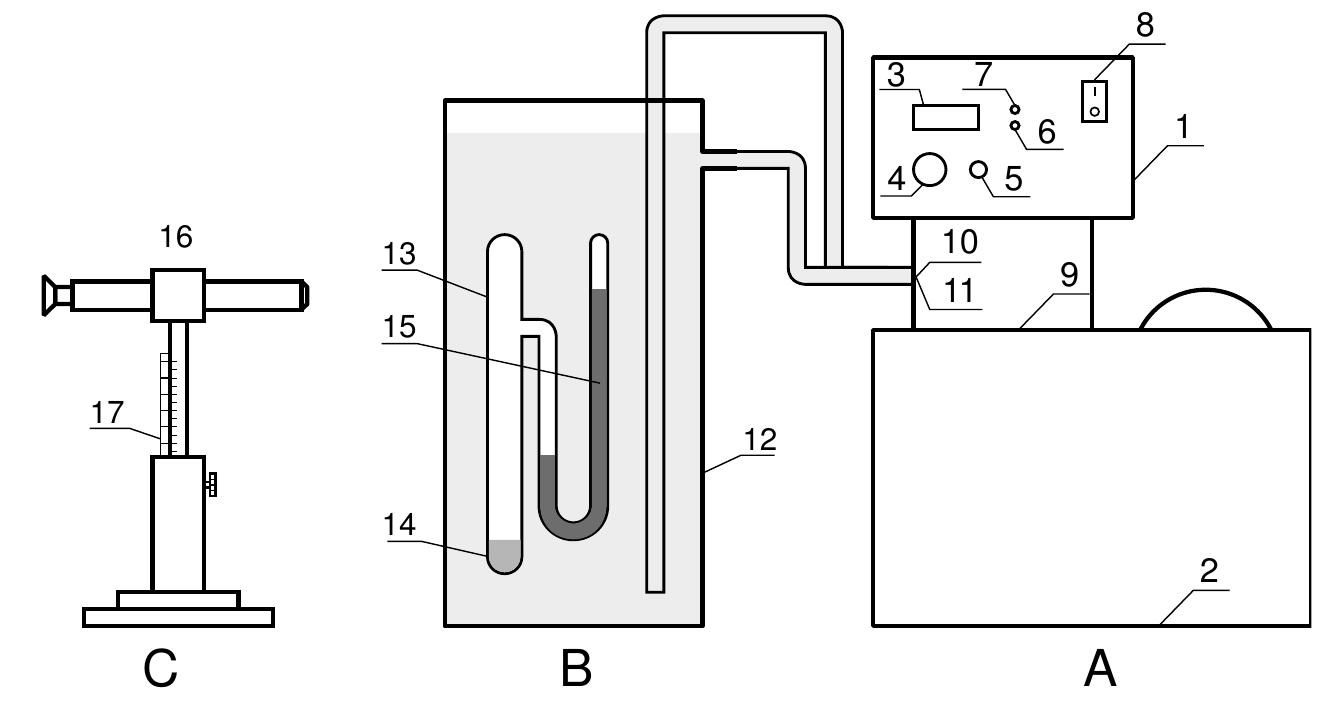
\includegraphics[width=0.8\linewidth]{img/cal.png}
\end{figure}

Прибор B представляет собой емкость 12, заполненную водой. В нее погрузили запаянный прибор 13 с
исследуемой жидкостью 14. Перед заполнением исследуемой жидкости воздух из запаянного прибора
был удален, так что над жидкостью находится ее насыщенный пар. Его давление определяется по ртутному
манометру 15, соединенному с емкостью 13. Численная величина давления измеряется по разности
показаний отсчётного микроскопа 16, настраиваемого последовательно на нижний и верхний
уровни столбика ртути манометра. Показания микроскопа снимаются по шкале 17.

Преимущество метода измернеия заключается в том, что при непосредственном методе измернеии
теплоты испарения опыты нужно проводить при неизменном давлении, и прибор не может быть запаян.
При этом невозможно обеспечить такую чистоту и неизменность экспериментальных условий.

Опиманный прибор обладает недостатком: термометр определяет температуру термостата, а не
исследуемой жидкости. Эти температуры близки лищь при медленном нагревании. Температуру в калориметре
следует менять не быстрее, чем на $1\;\text{K}$ в течении 1--3 минут.
